\section{Background prediction methods}

We use three background prediction methods to
estimate all backgrounds in the signal regions.
Events where a fake or heavy flavour lepton
fakes the signature of a di-lepton event (i.e. W+jets, Single Top,
QCD) are estimated using the fake rate method 
presented in Sec.~??.
Top pair, $WW$ and $Z \rightarrow \tau \tau$ events
are estimated from the $e\mu$-control sample (Sec.~\ref{sec:ofossubtraction}).
$Z\rightarrow ll$ ($l=e,\mu$) is estimated by
extrapolating in \HT and \MET.

\subsection{Different flavour subtraction} \label{sec:ofossubtraction}
Since all signal regions are expected to be  
dominated by $t\bar{t}$-production we use
the different flavour control sample ($e\mu$) to predict
backgrounds in which leptons uncorrelated in flavour are being produced.
It relies only on the knowledge of the ratio
of electron to muon reconstruction efficiency $r_{e\mu}$,
which we derive in Sec.~\ref{sec:eff}.

Under the assumption of lepton universality
The following two formulas hold for any background
where di-leptons are being produced uncorrelated 
(e.g. top-pairs events, $Z \rightarrow \tau^{+} \tau{-} \rightarrow 
l^{+} \l^-$, $WW$-production):
$$
n_{ee} = \frac12n_{e\mu}r_{\mu{}e}, \quad n_{\mu\mu} = \frac12\frac{n_{e\mu}}{r_{\mu{}e}}.
$$
A closure test of the method has been performed
using a simulated top-pair sample (including pileup) and
we observe a good agreement between prediction and MC truth:
$$
n_{ee} = ??.9 \pm 2.8 (\textnormal{stat.}) \; \textnormal{ (??.2 MC)}, 
\quad n_{\mu\mu} = ??.8 \pm 3.3 (\textnormal{stat.}) \; \textnormal{ (??.5 MC)}.
$$

Later in this note we are only interested
in an excess of $ee+\mu\mu$ and in this
extrapolation the ratio largely cancels
as long as the differences in lepton efficiencies are not
large.

One can define the quantity $S$
\be
    S = r_{\mu e} n_{ee} - n_{e\mu} + \frac{1}{r_{\mu e}} n_{\mu\mu}
\ee
to measure the total flavour assymmetry. It is expected
to be 0 for flavour symmetric processes,
but becomes positive for processes with higher
flavour correlated yield and negative for
processes with higher $e\mu$ yield.

\subsection{Z boson prediction} \label{sec:zprediction}

Backgrounds containing a real di-lepton pair of same flavour ($ee$ and $\mu\mu$)
are estimated by a partly data-driven extrapolation in \HT and \MET.
We start by extraction of the Z yield using a fit to the invariant
mass distribution in the preselection region ($\HT > 100$~GeV and $\MET>100$~GeV).
From the fit we extract a yield of 
\be
    n_{Z,control} = 5.4 \pm 3.4_{stat}
\ee
in $ee+\mu\mu$ modes. This yield is used
to derive a prediction in the signal regions
\be
    n_{Z,sig} = \epsilon_{\HT} \epsilon_{\MET} n_{Z,control},
\ee
where $\epsilon_{\HT}$ and $\epsilon_{\MET}$ describe
an extrapolation in \HT and \MET respectively.

The extrapolation in \HT is performed fully data-driven
by fitting the Z yield without \MET cut. For this
we select events for \HT>100~GeV, \HT>250~GeV, \HT>350~GeV
and \HT>600~GeV, which correspond to the \HT tresholds
used in various signal regions.
By using the ratio of the yields
in these regions we drive the efficiency of the \HT cut
\be
    \epsilon_{\HT} = \frac{n_{Z,\HT,signal}}{n_{Z,\HT,control}}.
\ee

The yields and efficiencies for all regions are summarised in Tab.~\ref{zHTExtrap}.

\begin{table}[hbtp]
\caption{Z yield in. \label{tab:zHTExtrap}}
\begin{center}
\begin{tabular}{l||c|c} \hline
\HT thresh. [GeV]   & Yield $n_{Z}$ &   $\epsilon_{\HT}$  \\\hline \hline
100 &  $3191\pm57$   &$1.$ \\
250 &  $158\pm13$   &$0.050 \pm 0.0057$ \\
350 &  $51\pm7$   &$0.016 \pm 0.0033$ \\
600 &  $21\pm5$   &$0.0066\pm 0.0021$ \\\hline
\end{tabular}
\end{center}
\end{table}

The extrapolation in \MET is performed 
from simulation after applying the \MET
and \HT cut of the preselection.
We find that suppression in \MET
is reduced after application of a higher
\HT selection, but the simulation is statistically
limited in this region.
The systematic uncertainty on this extrapolation
is assumed to be 50\%.

We derive a extrapolation factor of
\be
    \epsilon_{\MET,100 \rightarrow 150} = 0.5 \pm 0.25
\ee
for a \HT threshold of 250~GeV and 350~GeV.
For higher \MET selections no events are
selected according to simulation, 
thus we derive an upper limit on the number 
of events in that region.

Please note that this factor can also be
larger than one for a case where only
the \HT but not the \MET cut is
increased.

For all signal regions the expected Z yield
is rather low, so that a large systematic uncertainty
can be accommodated.

\subsection{Preselection region}

In the pre-selection region (\HT>100~GeV and \MET > 100~GeV)
we perform a full shape analysis of the different ($e\mu$) an same flavour ($ee$, $\mu\mu$)
lepton pairs.

A data to MC comparison of all same flavour events
is shown in Fig.~\ref{fig:sfosPre} for all same flavour
and in Fig.~\ref{fig:ofosPre} for the different flavour
pairs. It is seen that data and simulation do agree relatively good.

\begin{figure}[hbtp]
  \subfigure[]{\label{fig:sfosPre}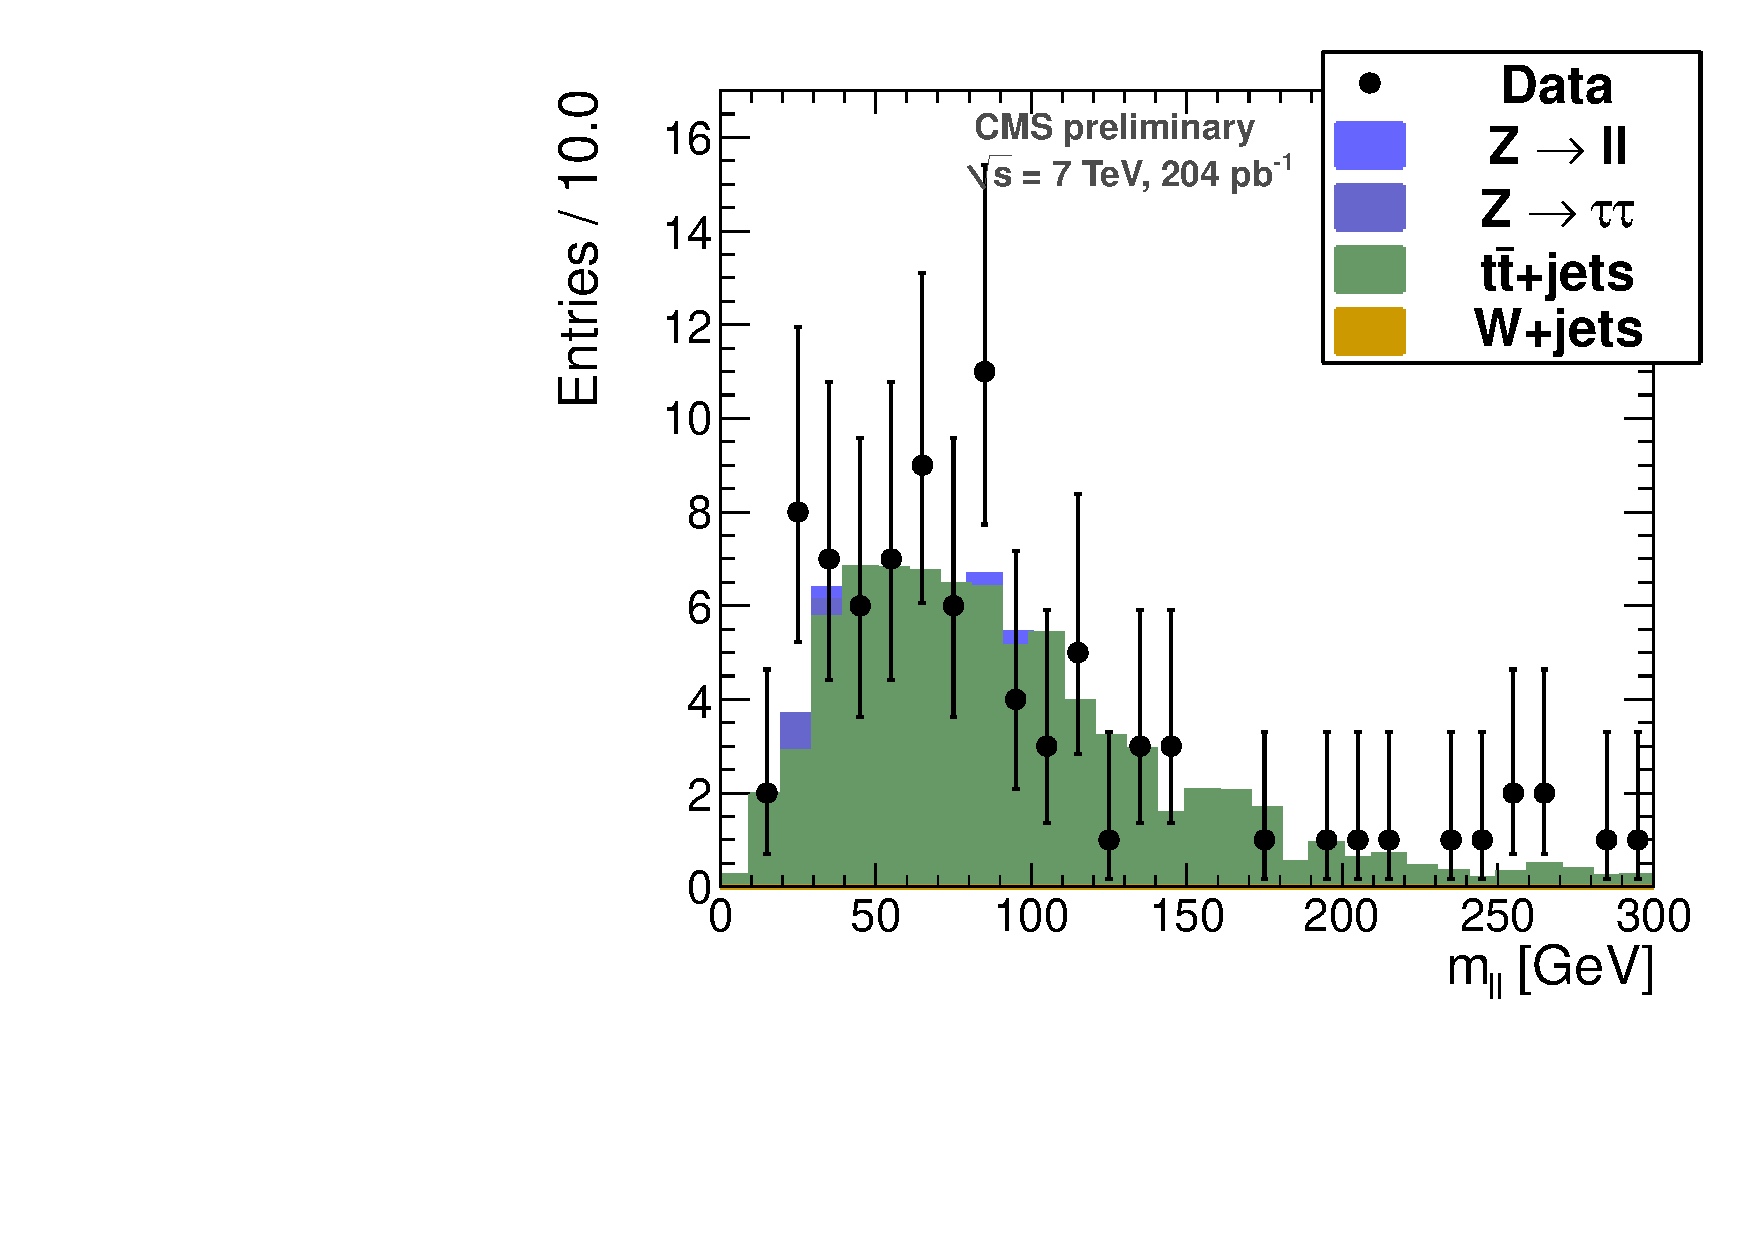
\includegraphics[width=0.49\textwidth]{Summer11_07_MC_pfLeptSusyCuts_Data_iOSSF_EEMuMu.pdf}}\hfill
  \subfigure[]{\label{fig:ofosPre}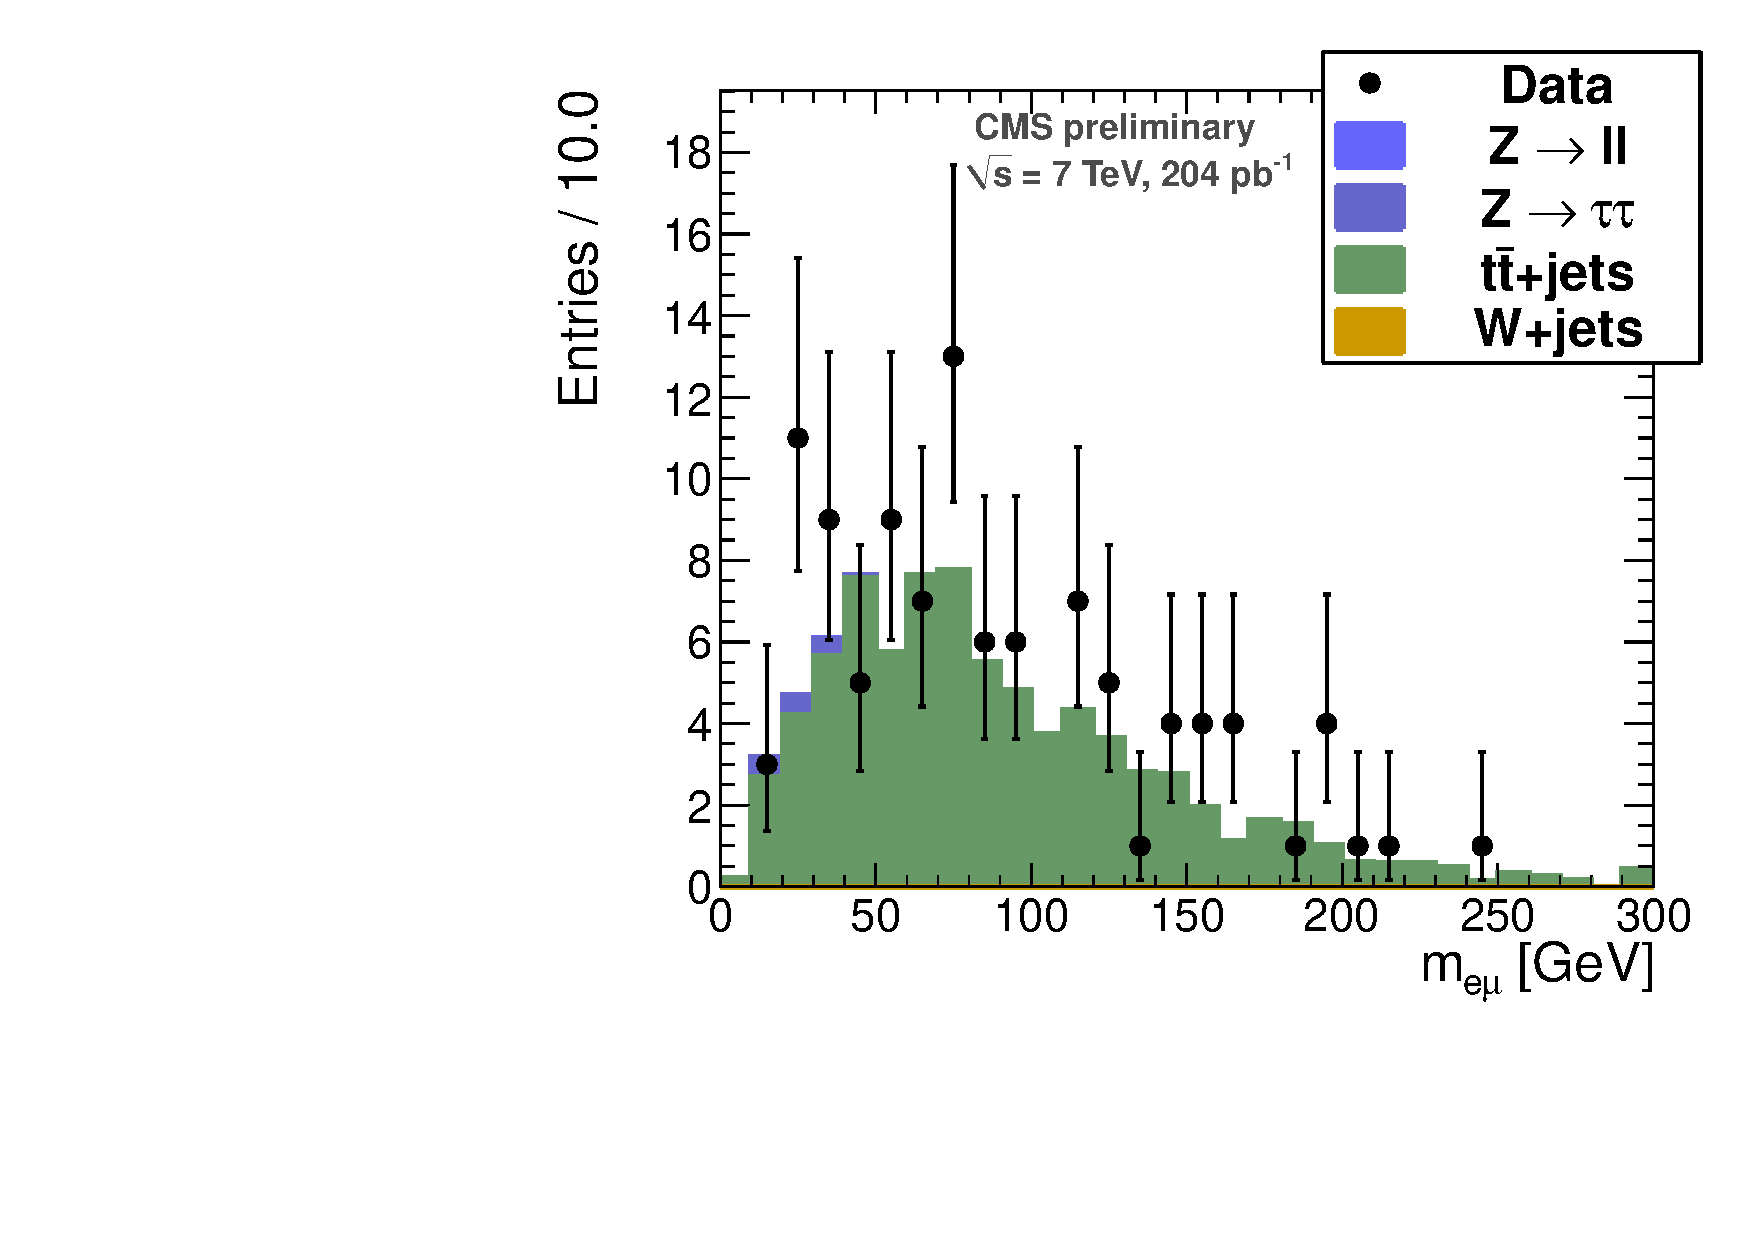
\includegraphics[width=0.49\textwidth]{Summer11_07_MC_pfLeptSusyCuts_Data_iOSOF_EMu.pdf}}\hfill
  \caption{Data to MC comparison for events in the pre-selection region ($HT>100$~GeV, $\MET> 100$~GeV)
  for an integrated luminosity of 204~\pbi. \subref{fig:sfosPre} shows the $ee+\mu\mu$-pairs and
 \subref{fig:ofosPre} $e\mu$-pairs.}
\end{figure}

In this region we perform a full shape analysis
of the same and different flavour lepton pairs.
The fit of the $e\mu$ lepton pairs is shown
in Fig.~\ref{fig:ofosFitPre}.
This background is described by 
\begin{equation}\label{eq:fit_bkg}
B(m_{ll}) = m_{ll}^{a} \cdot e^{-b\cdot m_{ll}}.
\end{equation}
The green band represents the statistical 
uncertainty on the shape.

The same flavour lepton pairs are fitted
by the background shape from $e\mu$
with the normalisation fixed within the 
statistical plus systematical uncertainty
from the $e\mu$-pairs.

For a potential signal the an edge model
is fitted and the Z contribution
is modelled by a Breit-Wigner convoluted 
with a Gaussian.

The fit of the $ee+\mu\mu$ lepton pairs is shown
in Fig.~\ref{fig:sfosFitPre}.

\begin{figure}[hbtp]
  \subfigure[]{\label{fig:sfosFitPre}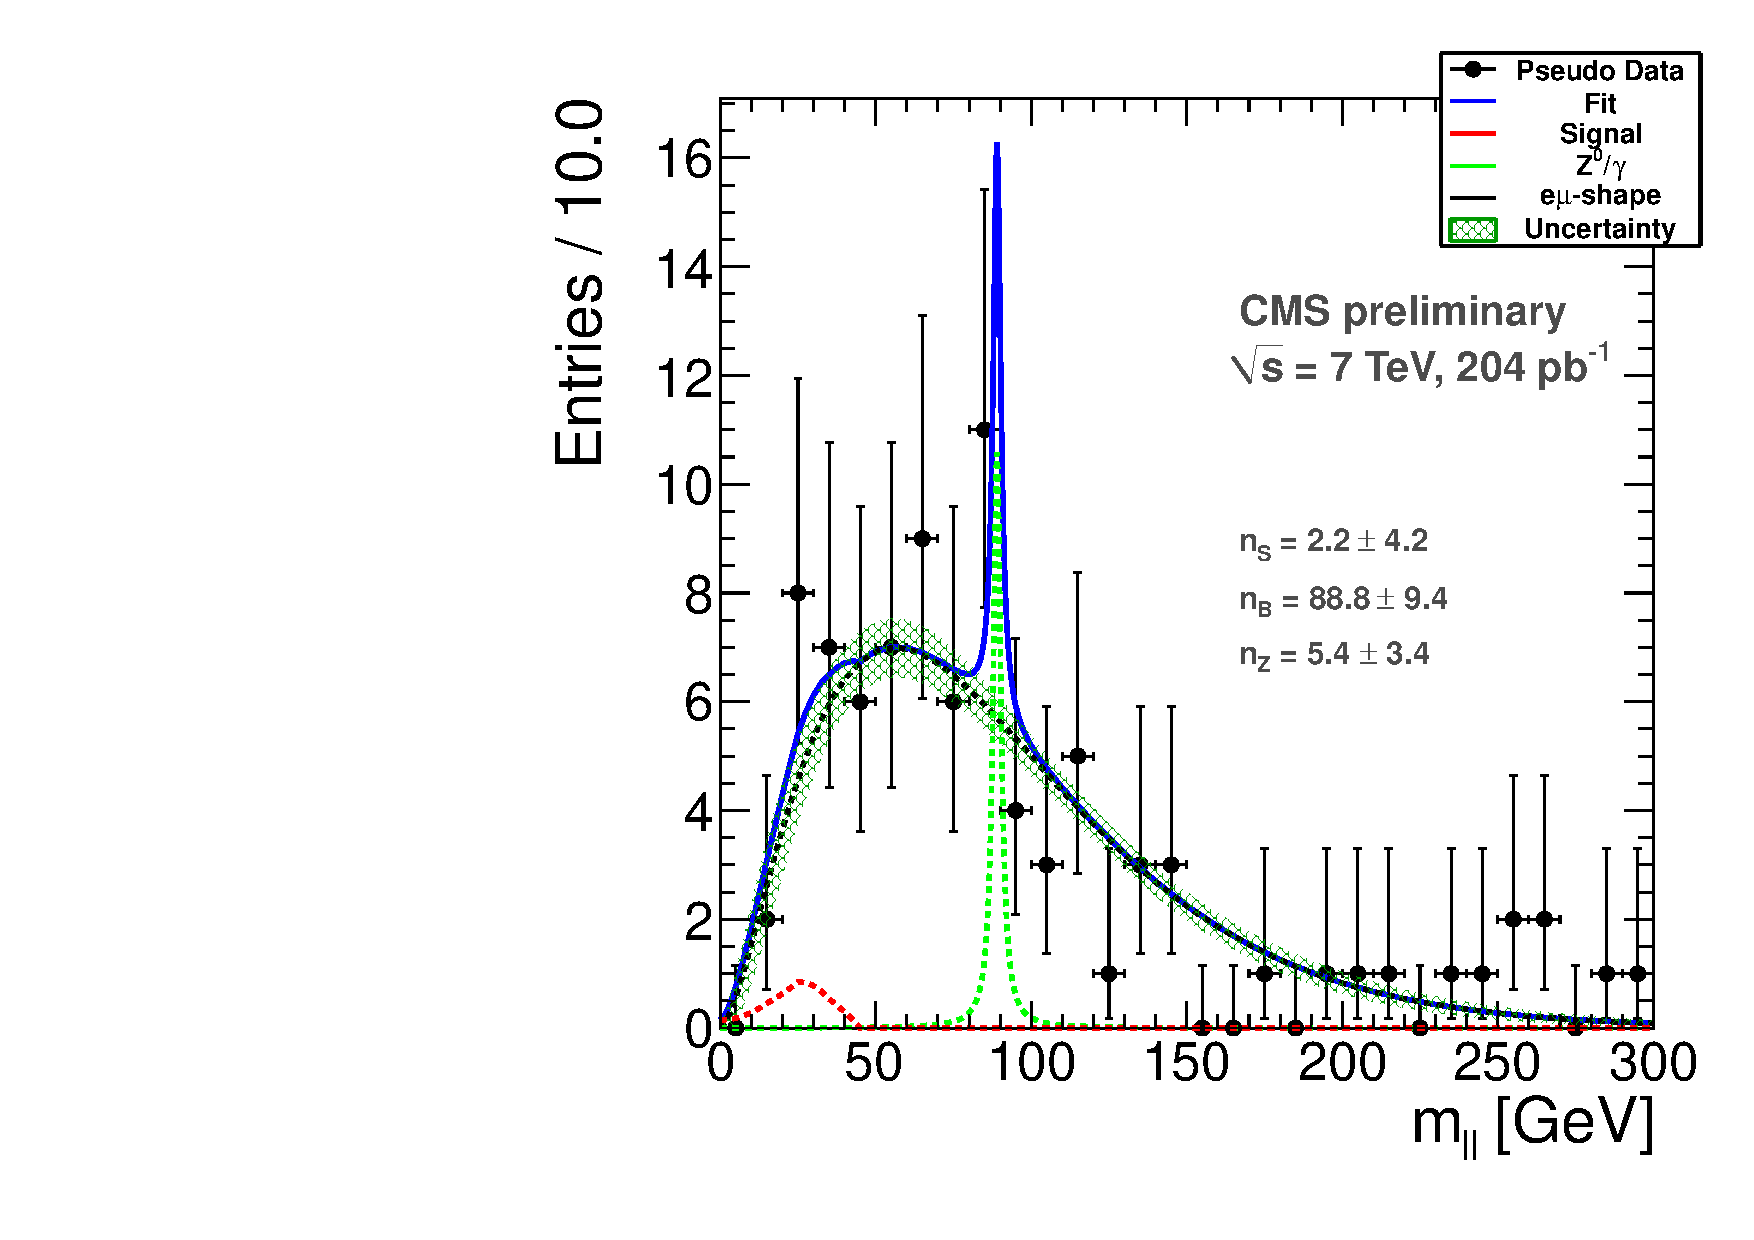
\includegraphics[width=0.49\textwidth]{fit2011_AG_Data.pdf}}\hfill
  \subfigure[]{\label{fig:ofosFitPre}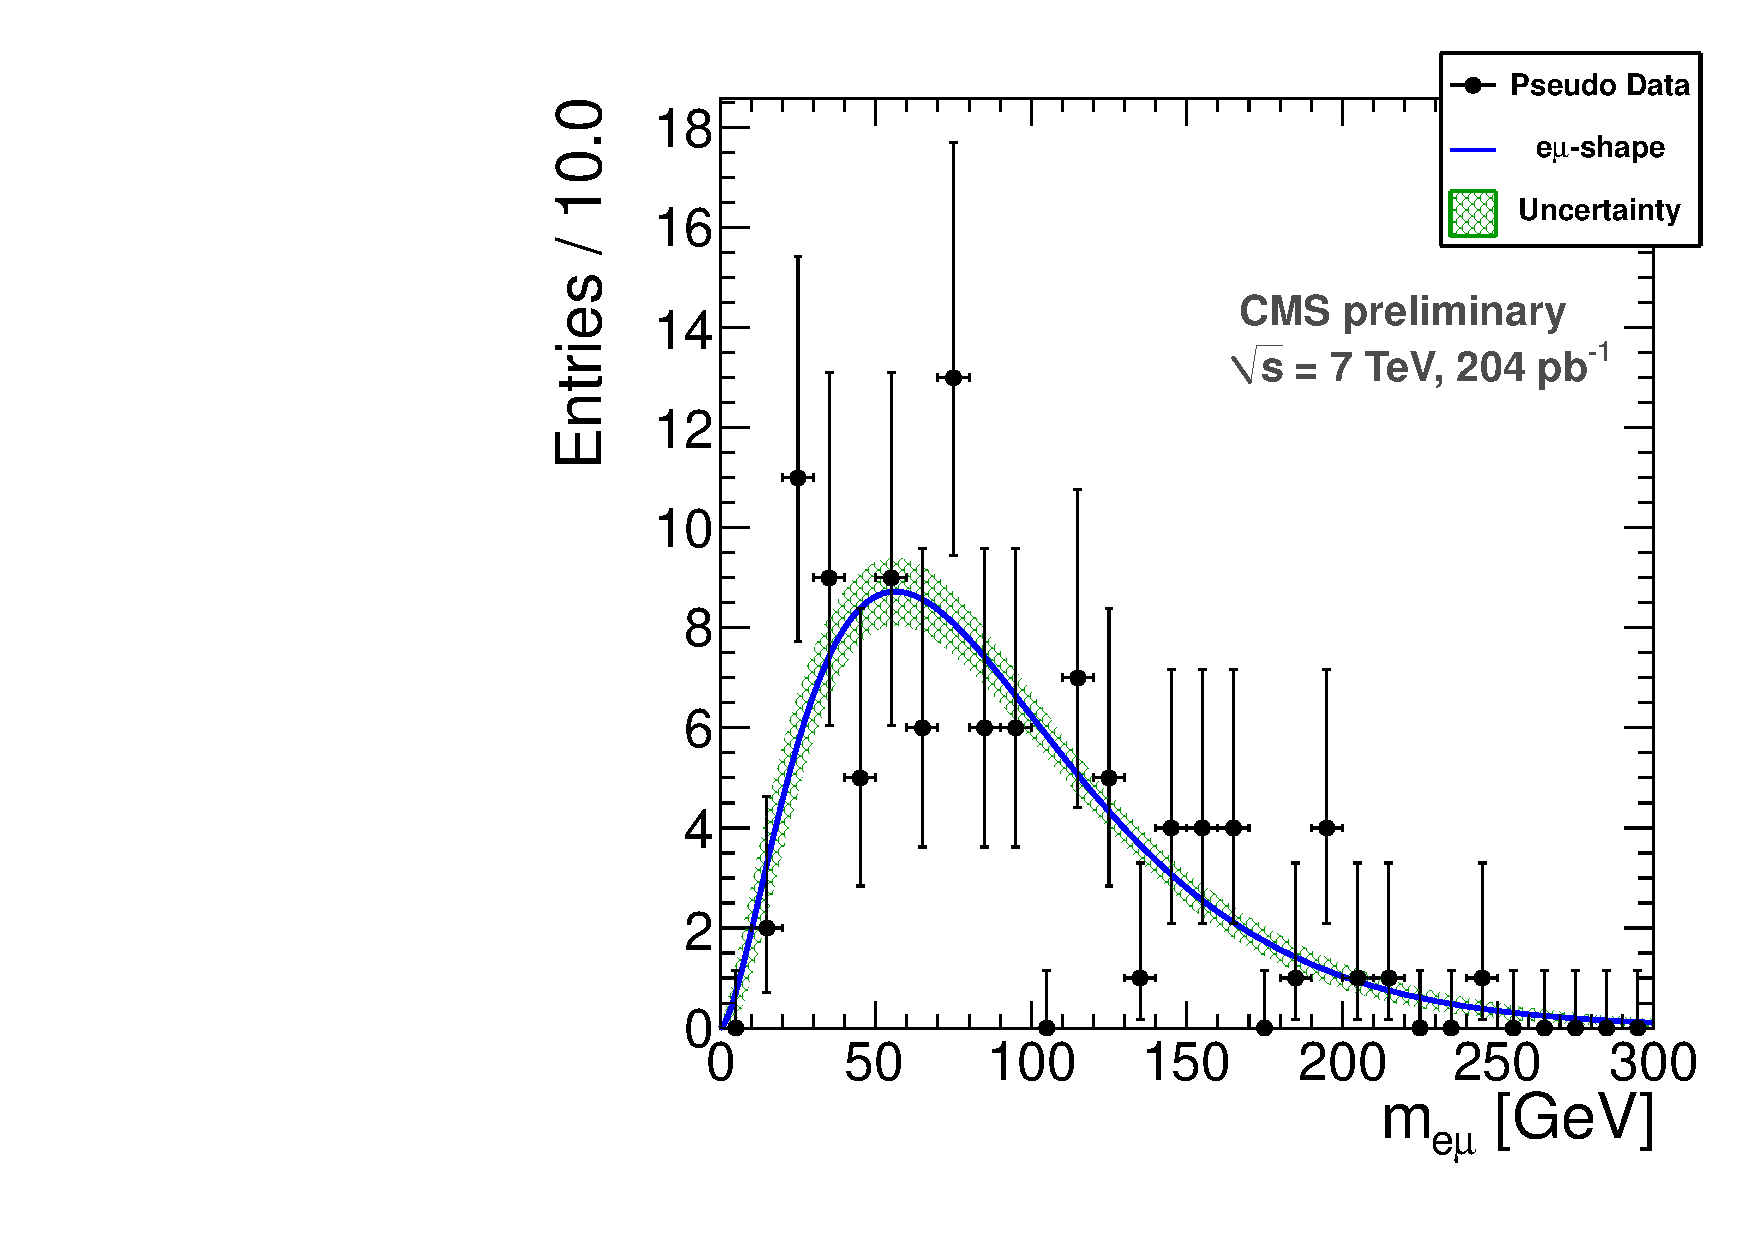
\includegraphics[width=0.49\textwidth]{fit2011OFOS_AG_Data.pdf}}\hfill
  \caption{Data to MC comparison for events in the pre-selection region ($HT>100$~GeV, $\MET> 100$~GeV)
  for an integrated luminosity of 204~\pbi. \subref{fig:sfosPre} shows the $ee+\mu\mu$-pairs and
 \subref{fig:ofosPre} $e\mu$-pairs.}
\end{figure}

It is seen that no significant contribution
above the background is observed.
